\documentclass[xcolor=dvipsnames,table]{beamer}

\usepackage{latexsym}
\usepackage[utf8]{inputenc}
\usepackage[brazil]{babel}
\usepackage{amssymb}
\usepackage{amsmath}
\usepackage{stmaryrd}
\usepackage{fancybox}
\usepackage{datetime}
\usepackage[T1]{fontenc}
\usepackage{graphicx}
\usepackage{graphics}
\usepackage{url}
\usepackage{algorithmic}
\usepackage{algorithm}
\usepackage{acronym}
\usepackage{array}

\newtheorem{definicao}{Definio}
\newcommand{\tab}{\hspace*{2em}}

\mode<presentation>
{
  \definecolor{colortexto}{RGB}{0,0,0}
 
  \setbeamertemplate{background canvas}[vertical shading][ bottom=white!10,top=white!10]
  \setbeamercolor{normal text}{fg=colortexto} 

  \usetheme{Warsaw}
}

\title{Apresentação da disciplina} 

\author{
  Esdras Lins Bispo Jr. \\ \url{bispojr@ufg.br}
  } 
 \institute{
  Teoria da Computação \\Bacharelado em Ciência da Computação}
\date{\textbf{02 de maio de 2015} }

\logo{
\includegraphics[width=1cm]{images/ufgJataiLogo.png}}

\begin{document}

	\begin{frame}
		\titlepage
	\end{frame}

	\AtBeginSection{
		\begin{frame}{Sumário}%[allowframebreaks]{Sumário}
    		\tableofcontents[currentsection]
    		%\tableofcontents[currentsection, hideothersubsections]
		\end{frame}
	}

	\begin{frame}{Plano de Aula}
		\tableofcontents
		%\tableofcontents[hideallsubsections]
	\end{frame}
	
	\section{Sobre a Disciplina}
	\subsection{Professor}
	\begin{frame}{Professor}
		\begin{columns}
			\column{.4\textwidth}  		
		  		\begin{center}
		    		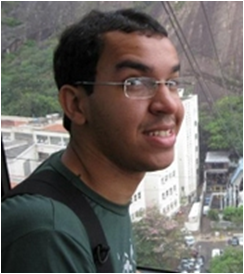
\includegraphics[height=.5\textheight]{images/esdras.png}
		  		\end{center}
			\column{.6 \textwidth}  		
				\begin{block}{Formação}
					\begin{center}
						{\normalsize {\bf Bacharel} em Sistemas de Informação\\
						{\bf Mestre} e {\bf Doutorando} em Representação Conhecimento (IA)}
					\end{center}
				\end{block}		  		
		  		\begin{block}{Quem?}
		  			\begin{center}
						{\bf Esdras Lins Bispo Junior} \\ Recife, Pernambuco.
					\end{center}
				\end{block}
		\end{columns}
	\end{frame}
	
	\begin{frame}{Professor}
		\begin{center}
    		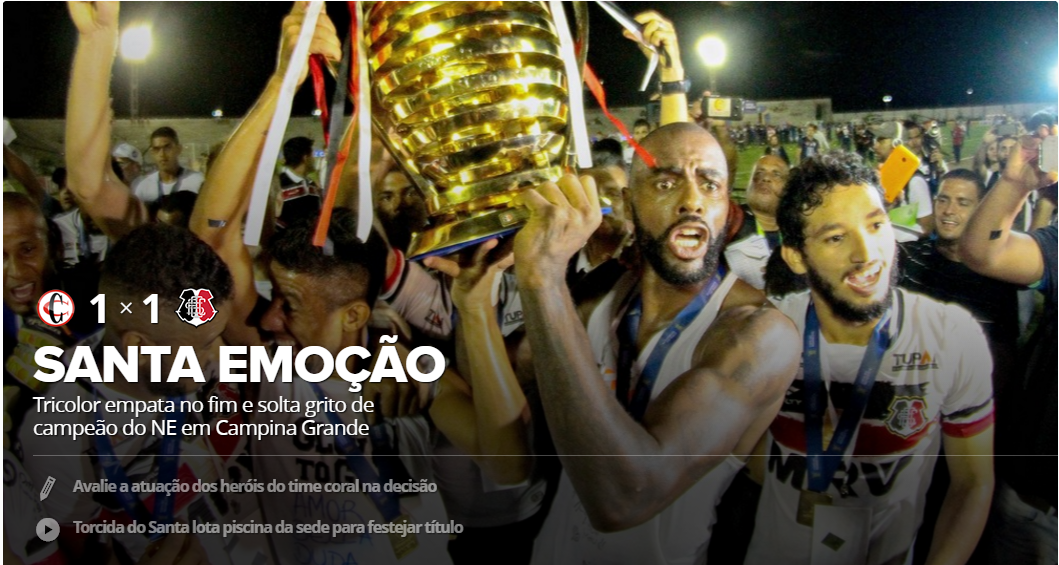
\includegraphics[height=.65\textheight]{images/santa.png}
  		\end{center}
	\end{frame}
	
	\subsection{Informações Importantes}
	\begin{frame}{Informações Importantes}
		\begin{block}{Professor}
			\begin{itemize}
				\item Esdras Lins Bispo Jr.
				\item \url{bispojr@ufg.br}
				\item Sala 18, 1º Andar (Bloco Novo dos Professores)
			\end{itemize}
		\end{block}
	\end{frame}	
	
	\begin{frame}{Informações Importantes}
		\begin{block}{Disciplina}
			\begin{itemize}
				\item Teoria da Computação
				\item 09h30-11h10 (Segunda, LSD)\\
					  09h30-11h10 (Terça, LSD)
				\item Dúvidas: 09h30 - 11h10 (Quarta)\\
					  {\color{red}[é necessário confirmação comigo]}
				\item \url{www.facebook.com/groups/teocomp.rej.2016.1/}
			\end{itemize}
		\end{block}
	\end{frame}
	
	\begin{frame}{Informações Importantes}
		\begin{block}{Metodologia}
			\begin{itemize}
				\item Aulas expositivas;
				\item Testes;
				\item Prova;
				\item Exercícios.
			\end{itemize}
		\end{block}
	\end{frame}
	
	\begin{frame}{Informações Importantes}
		\begin{block}{Testes}
			\begin{itemize}
				\item Teste 1 $\Rightarrow$ 20\% da pontuação total (16 de maio);
				\item Teste 2 $\Rightarrow$ 20\% da pontuação total (13 de junho);
				\item Teste 3 $\Rightarrow$ 20\% da pontuação total (28 de junho);
				\item Teste 4 $\Rightarrow$  20\% da pontuação total (08 de agosto).
			\end{itemize}
		\end{block}
		\begin{block}{Avaliação}
			\begin{itemize}
				\item Prova $\Rightarrow$  20\% da pontuação total (16 e 30 de agosto).
			\end{itemize}
		\end{block}
		\begin{block}{Exercícios [Bônus]}
			\begin{itemize}
				\item Somatório dos exercícios.
			\end{itemize}
		\end{block}
	\end{frame}
    
    \begin{frame}{Informações Importantes}
		\begin{block}{Exercícios-Bônus}
			\begin{itemize}
				\item Semanalmente serão disponibilizados exercícios-bônus (EB) valendo 0,5 ponto na média (segunda-feira, normalmente); \pause
                \item Será dado um prazo para as candidaturas\\
                (normalmente um dia); \pause
                \item Será dada prioridade às candidaturas aos seguintes alunos: \pause
                	\begin{enumerate}
                    	\item Respondeu a nenhum EB; \pause
                        \item Respondeu a um EB; \pause
                        \item Respondeu a dois EBs; \pause
                        \item e assim por diante.
                    \end{enumerate} \pause
                \item Haverá sorteio entre candidatos dentro da mesma prioridade; \pause
            	\item Uma semana após, o candidato apresentará a sua resposta [texto escrito e slides] (normalmente na segunda, 11h30).
			\end{itemize}
		\end{block}
	\end{frame}
	
	\begin{frame}{Informações Importantes}
		\begin{block}{Avaliação}
			O cálculo da média final será dada da seguinte forma:
			\begin{itemize}
				\item MF = MIN(10, PONT)
			\end{itemize}
			em que MIN representa o mínimo entre dois valores e PONT representa a pontuação total obtida em toda a disciplina.
		\end{block} \pause
		\begin{exampleblock}{Previsão de Término das Atividades}
			06 de setembro de 2016
		\end{exampleblock}
	\end{frame}

	\begin{frame}{Informações Importantes}
		\begin{block}{Conteúdo do Curso}
			\begin{enumerate}
				\item Introdução à Teoria da Computação;
				\item Modelos de Computação;
				\item Problemas decidíveis;
				\item Problemas indecidíveis;
				\item Complexidade de tempo;
				\item NP-Completude;
				\item Tópicos Avançados.
			\end{enumerate}
		\end{block}
	\end{frame}

%------------------------------------------
	\section{Pensamento}
	\begin{frame}{Pensamento}
  		\begin{center}
    		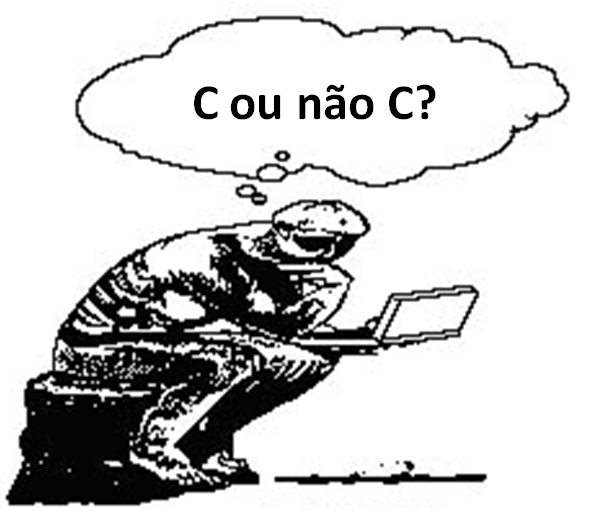
\includegraphics[width=7cm]{images/pensamento.png}
  		\end{center}
	\end{frame}
	
	\begin{frame}{Pensamento}
		\begin{columns}
			\column{.4\textwidth}  		
		  		\begin{center}
		    		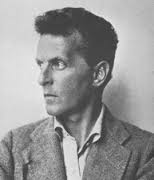
\includegraphics[height=.5\textheight]{images/wittgenstein.jpg}
		  		\end{center}
			\column{.6\textwidth}  		
				\begin{block}{Frase}
					\begin{center}
						{\large Os limites do meu conhecimento são os limites do meu mundo.}
					\end{center}
				\end{block}		  		
		  		\begin{block}{Quem?}
		  			\begin{center}
						{\bf Ludwig Wittgenstein (1889-1951)} \\ Filósofo austríaco.
					\end{center}
				\end{block}
		\end{columns}
	\end{frame}
%------------------------------------------
	\section{Introdução}
	\subsection{O que é Teoria da Computação?}
	\begin{frame}{O que é Teoria da Computação?}
		Pode ser dividida em três grandes áreas:
		\begin{itemize}
			\item Teoria dos Autômatos;
			\item Teoria da Computabilidade;
			\item Teoria da Complexidade.	
		\end{itemize}\pause
		São interligadas pela pergunta:
		\begin{block}{}
			Quais são as capacidades e limitações fundamentais dos computadores?
		\end{block}
	\end{frame}
	
	\begin{frame}{O que é Teoria da Computação?}
		\begin{block}{Teoria dos Autômatos}
			Quais são as definições e propriedades dos modelos matemáticos de computação?
		\end{block} \pause
		\begin{block}{Teoria da Computabilidade}
			O que faz alguns problemas serem solúveis e outros não?		
		\end{block} \pause
		\begin{block}{Teoria da Complexidade}
			O que faz alguns problemas serem computacionalmente difíceis e outros fáceis?
		\end{block}
	\end{frame}
	
	\section{Máquina de Turing}
	\begin{frame}{Modelos Básicos Computacionais}
		\begin{block}{AFDs, AFNs, e Expressões Regulares}
			\begin{itemize}
				\item Potencialidades: reconhecem linguagens como $({\tt 10} \cup {\tt 1})^*$;
				\item Fragilidades: não reconhecem linguagens como $A = \{ {\tt 0}^n {\tt 1}^n \mbox{ | } n \geq 0 \mbox{ e } n \in \mathbb{N} \}$.
			\end{itemize}
		\end{block} \pause
		\begin{block}{GLCs e Autômatos com Pilha}
			\begin{itemize}
				\item Potencialidades: reconhecem linguagens como $A = \{ {\tt 0}^n {\tt 1}^n \mbox{ | } n \geq 0 \mbox{ e } n \in \mathbb{N} \}$;
				\item Fragilidades: não reconhecem linguagens como $A = \{ {\tt a}^n {\tt b}^n {\tt c}^n\mbox{ | } n \geq 0 \mbox{ e } n \in \mathbb{N} \}$.
			\end{itemize}
		\end{block} \pause
		\begin{alertblock}{}
			Portanto são bem restritos para servir de modelo de computadores de propósito geral.
		\end{alertblock}
	\end{frame}
	
	\begin{frame}{Máquinas de Turing (MT)}
		\begin{itemize}
			\item Modelo mais poderoso que GLCs e AFDs; \pause
			\item Turing, 1936; \pause
			\item Características importantes:
				\begin{enumerate}
					\item faz tudo o que um computador real pode fazer;
					\item existem certos problemas que uma MT não pode resolver.
				\end{enumerate}				 
			
		\end{itemize}
	\end{frame}
	
	\begin{frame}{Máquinas de Turing (MT)}
		\begin{center}
			
\includegraphics[height=4cm]{images/harry.png}
			
			- {\it Salaminh salah-mês}... tranforme as figuras em inglês!
		\end{center}
	\end{frame}	
	
	\begin{frame}{Máquinas de Turing (MT)}
		\begin{center}
			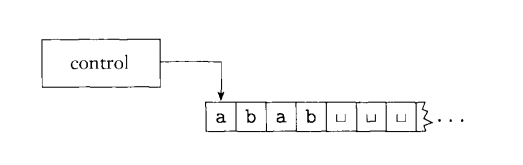
\includegraphics[height=3.5cm]{images/fig31.png}
		\end{center}
	\end{frame}
	
	\begin{frame}{Máquinas de Turing (MT)}
		\begin{block}{Diferenças entre MT e AFDs}
			\begin{itemize}
				\item Uma MT pode tanto escrever sobre a fita quanto ler a partir dela;
				\item A cabeça de leitura-escrita pode mover-se tanto para a esquerda quanto para a direita;
				\item A fita é infinita;
				\item Os estados especiais para rejeitar e aceitar fazem efeito imediatamente.
			\end{itemize}
		\end{block}
	\end{frame}
	
	\begin{frame}{Máquinas de Turing (MT)}
		\begin{block}{Construindo uma MT}
			\begin{center}
			Construir $M_1$ que reconheça a linguagem $B = \{ \omega \# \omega \mbox{ | } \omega \in \{ 0, 1 \}^* \}$.
			\end{center}
		\end{block}
	\end{frame}
	
	\begin{frame}{Máquinas de Turing (MT)}
		\begin{block}{Descrição de $M_1$}
			$M_1 =$ ``Sobre a cadeia de entrada $\omega$:
			\begin{enumerate}
				\item Faça um zigue-zague ao longo da fita checando posições correspondentes de ambos os lados do símbolo $\#$ para verificar se elas contêm o mesmo símbolo. Se elas não contêm, ou se nenhum $\#$ for encontrado, {\it rejeite}. Marque os símbolos à medida que eles são verificados para manter registro de quais símbolos têm correspondência.
				\item Quando todos os símbolos à esquerda do $\#$ tiverem sido marcados, verifique a existência de algum símbolo remanecente à direta do $\#$. Se resta algum símbolo, {\it rejeite}; caso contrário, {\it aceite}.
			\end{enumerate}
		\end{block}
	\end{frame}
	
	\begin{frame}{Máquinas de Turing (MT)}
		\begin{center}
			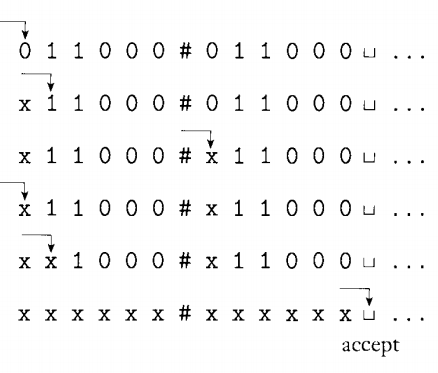
\includegraphics[height=6cm]{images/fig32.png}
		\end{center}
	\end{frame}	
	
	\begin{frame}{Máquinas de Turing (MT)}
		Uma {\bf máquina de Turing} é uma 7-upla $(Q, \Sigma, \Gamma, \delta, q_0, q_{aceita}, q_{rejeita})$, de forma que $Q, \Sigma, \Gamma$ são todos conjuntos finitos e

		\begin{enumerate}
			\item $Q$ é o conjunto de estados,
			\item $\Sigma$ é o alfabeto de entrada sem o {\bf símbolo branco} $\sqcup$,
			\item $\Gamma$ é o alfabeto da fita, em que $\sqcup \in \Gamma$ e $\Sigma \subseteq \Gamma$,
			\item $\delta : Q \times \Gamma \rightarrow Q \times \Gamma \times \{E, D\}$ é a função de transição,
			\item $q_0 \in Q$ é o estado inicial,
			\item $q_{aceita} \in Q$ é o estado de aceitação, e
			\item $q_{rejeita} \in Q$ é o estado de rejeição, em que $q_{rejeita} \not= q_{aceita}$.
		\end{enumerate}
	\end{frame}
	
	\begin{frame}{Bônus (0,5 pt)}
		\begin{block}{Desafio}
			\begin{itemize}
				\item Mostre que a linguagem $B = \{ \omega \# \omega \mbox{ | } \omega \in \{ 0, 1 \}^* \}$ \\não é regular; \pause
                \item Candidaturas até amanhã (03 de maio, 09h30); \pause
                \item Apresentação e resposta por escrito $\rightarrow$ \\segunda (10 de maio, 11h30); \pause
                \item 20 minutos de apresentação.
			\end{itemize}
		\end{block} \pause
        \begin{block}{Livro}
			SIPSER, M. {\bf Introdução à Teoria da Computação}, 2a Edição, Editora Thomson Learning, 2011. \color{blue}{\bf Código Bib.: [004 SIP/int]}.
		\end{block}
	\end{frame}
	
	\begin{frame}
		\titlepage
	\end{frame}
	
\end{document}